%% magnet.tex  SC-Magnet  Kin, Achim 20p     
 
\title{}
\author{Robert Lambiase \and Kin Yip}
\date{20/08/2015}

\section{\rmfamily {sPhenix Magnet Power Supply Description}}
\label{Magnet_Power_Supply_and_Quench_Proection}
%\begin{center}
%{\rmfamily {\large Bob Lambiase}}
%\end{center}
%\begin{center}
%{\rmfamily {\large August 20, 2015}}
%\end{center}


\subsection{\rmfamily {\large Elements of the Power Supply System}}

{\rmfamily { Figure~\ref{fig:magnet_circuit} shows the main elements of the sPhenix powering system.}}

\begin{figure}[!hbt]
 \begin{center}
   {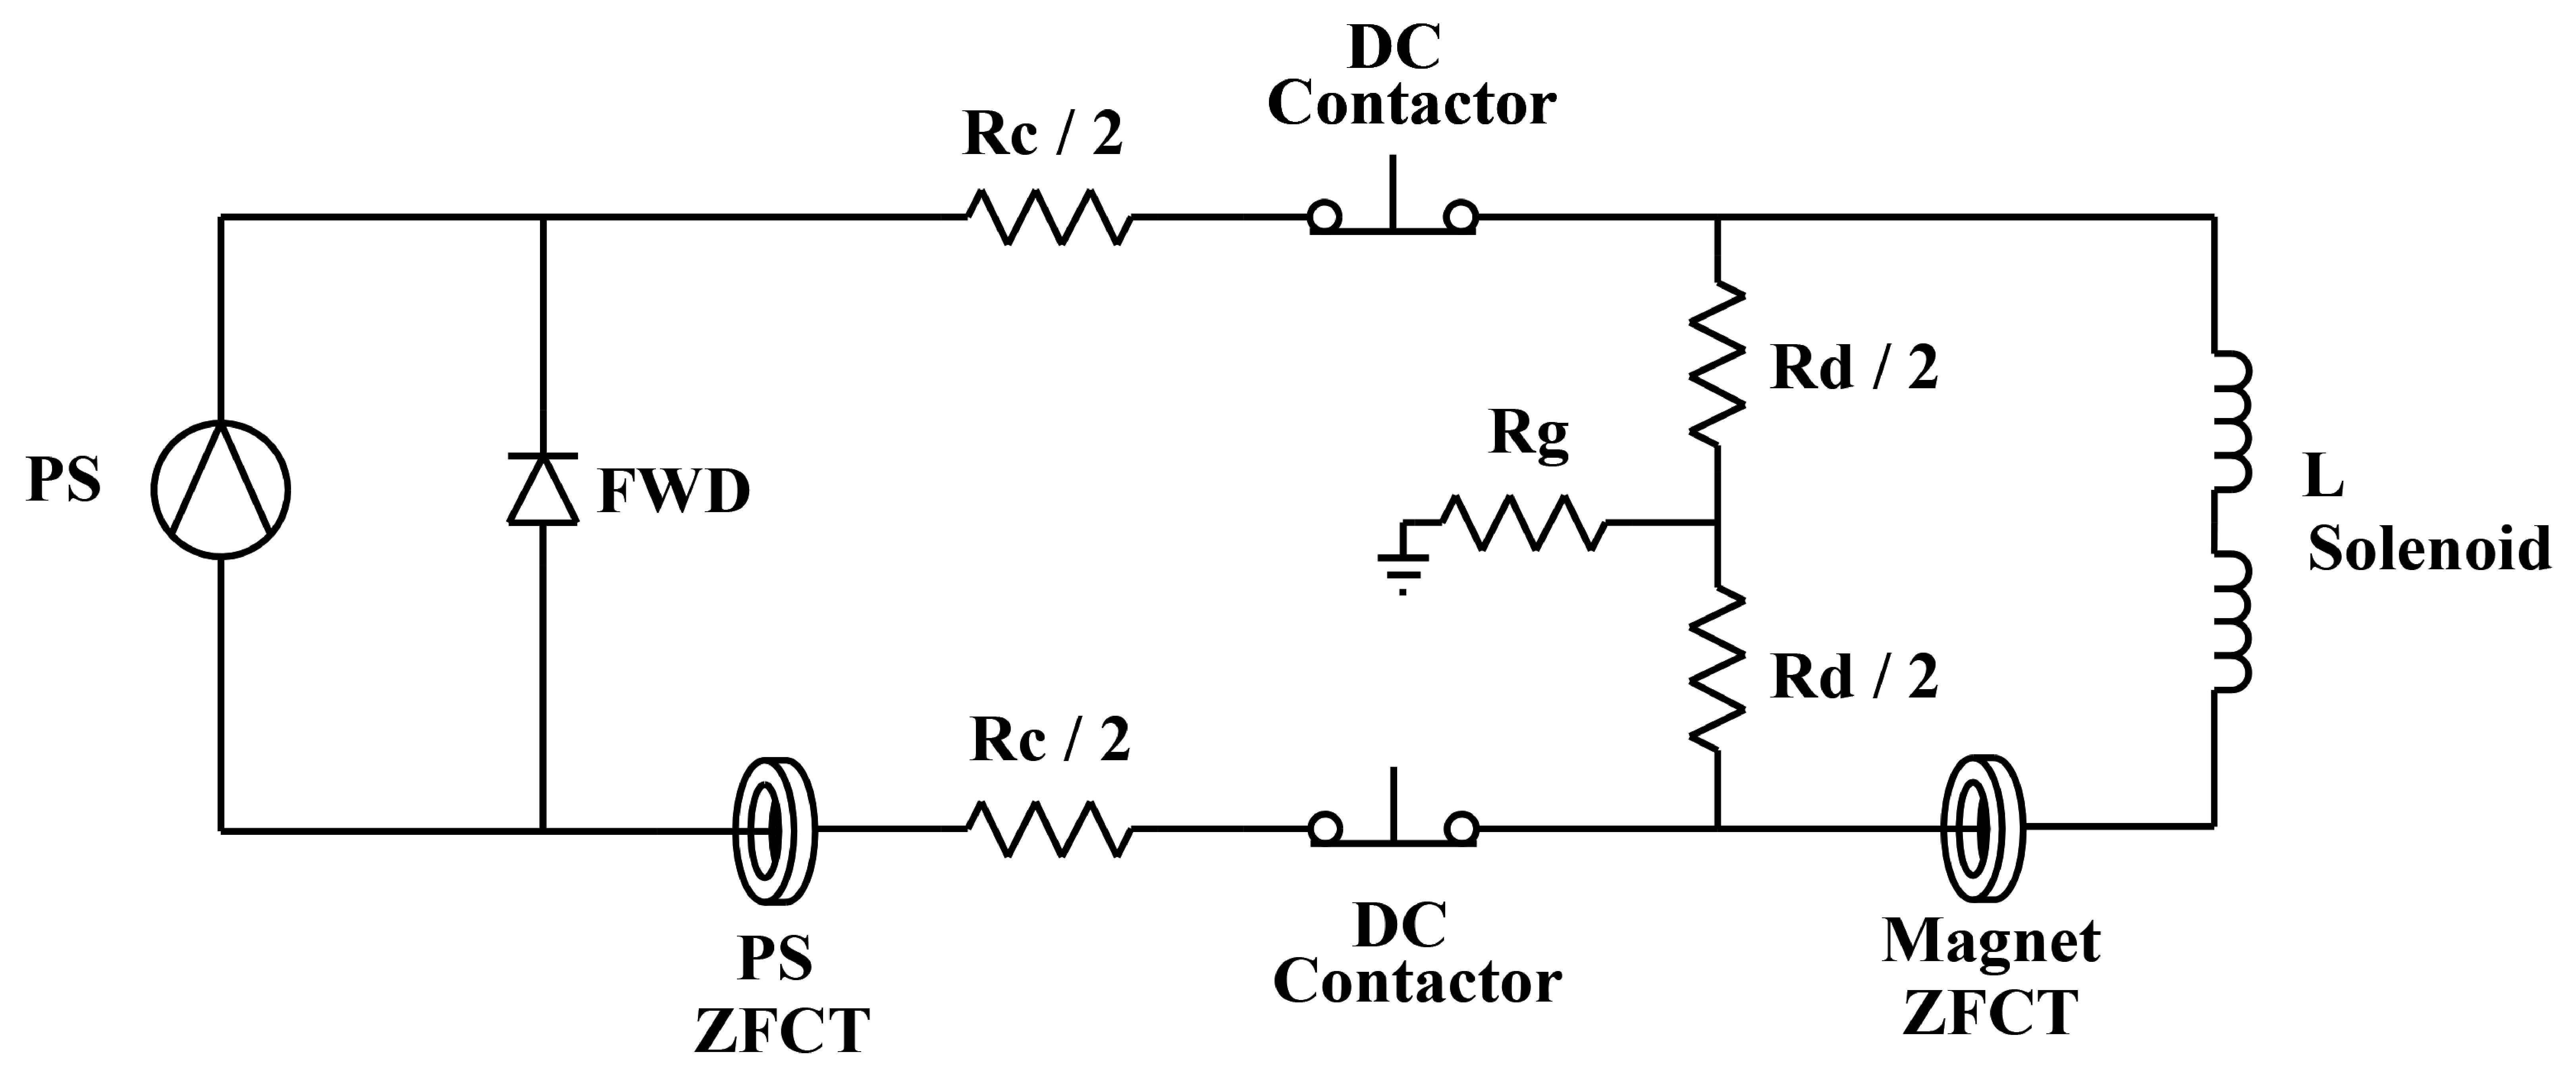
\includegraphics[width=\linewidth]{figs/PS_Arrangement.pdf}}
%   \raisebox{4pt}{\includegraphics[width=0.7\linewidth]{ps_arrangement.png}}
%    \caption[Probing Systems]{Probing systems example....
    \label{fig:magnet_circuit}
 \end{center}
\end{figure}

\renewcommand{\theenumi}{\Alph{enumi}}
\begin{enumerate}
\item {\rmfamily { L}~{  Solenoid}{  = 2.5}{  Hy}\\
\\
{ The solenoid is represented as two inductors in series, as it constructed in two layers.  The connection between the two layers is brought outside the solenoid, to be used by the quench protection system.  It is close, but not exactly, a true center tap.  The two layers have slightly different number of turns (531 vs. 536), and the inner winding has greater capacitive coupling to the }{ support cylinder. }{ }}

\item {\rmfamily { Rd = 68 m$\Omega$}\\
\\
{Rd is energy dump resistor, used to quickly reduce the current in the solenoid if a quench is detected.  This minimizes the energy absorbed within the solenoid.  It is split in two, with a soft reference to ground at the center point.}{   With this split, the voltage on either side of the solenoid to ground is only half the full dump voltage. }{ }}

\item {\rmfamily { Rg = 67 m$\Omega$} \\
\\
{ Rg limits the ground current, should the coil fault to ground.  The voltage across Rg is monitored by a ground fault detector.}{ }}

\item {\rmfamily { Magnet ZFCT} \\
\\{ The magnet zero flux current transducer (ZFCT)  accurately measures the current into the solenoid.  It differs from the power supply current by the current flowing through the dump resistor.  For this reason, this is the ZFCT used to regulate the current in the power supply.}{ }}

\item {\rmfamily { DC Contactor}\\
\\
{ In the event of a quench, the DC contactors are opened, and the power supply is disconnected from the solenoid.  The full solenoid current is then directed through the energy dump resistor. }{ }}

\item {\rmfamily { Rc = 1.25 m$\Omega$  (SLAC Configuration)}\\
\\
{ Rc is the cable resistance.  It determines the time to ramp down the }{ current through}{  the freewheeling diode (FWD) when the power supply turns off.}{ }}

\item {\rmfamily { PS ZFCT}\\
\\
{ The power supply ZFCT is for testing purposes, as it does not represent the solenoid current as accurately as the magnet ZFCT.}{ }}

\item {\rmfamily { FWD}\\
\\
{ The freewheeling diode (FWD) provides a current path when the power supply is turned off or trips.  }{ }}

\item {\rmfamily { PS}\\
\\{ The power supply (PS) nominally operates 4.6 kA and less than 20V.  The unit is manufactured to operate up to 8 kA and }{ 40 V.  Taps on the input transformer are used to reduce the maximum operating voltage.}}
\end{enumerate}




\newpage

\subsection {\rmfamily { Operating Conditions}{ }}
\begin{enumerate}
\item {\rmfamily { Ramping Up to Full Current}\\
\\
{ Under the conditions where the current is ramped from zero to 4.6 kA at a rate of 2.5~A/sec:}{ }}
\begin{enumerate}
\item {\rmfamily { The time to reach full current is (4,600 A) / (2.5 A/sec) = 1,840~seconds }\\
  { = 30.7~minutes.}{ }}
\item {\rmfamily { The voltage across the magnet is V}{ m}{  = L di/dt = 2.5 Hy x 2.5 A/sec = 6.25 V.}{ }}
\item {\rmfamily { The current through Rd is }{ Vm / Rd = }{ 6.25 V / 68 m$\Omega$ = 92 Amps}{ }}
\item {\rmfamily { The peak power supply voltage is Rc (}{ Im + Id) + Vm }
  \\ { = 1.25 m$\Omega$ (4.600 + 92) + 6.25 = 12.1 V.}{ }}
\end{enumerate}

\item {\rmfamily { Slow Discharge through FWD}{  and Rc}{ }}
\begin{enumerate}
\item {\rmfamily { Time constant $\tau$ = L / R}{ c}{  = 2.5 Hy / 1.25 m$\Omega$ = 2,000 seconds = 33.3 minutes}{ }}
\item {\rmfamily { Time to decay  from 4.6 kA to 100 A (as an example), }\\
{ Td = -$\tau$ ln(I / Io) = -33.3 ln (100 / 4,600) = 127.5 minutes = 2.1 hours}{ }}
\end{enumerate}

\item {\rmfamily { Fast Discharge through Dump Resistor}{ }}

\begin{enumerate}
\item {\rmfamily { Time constant $\tau$ = L / Rd = 2.5 Hy / 68 m$\Omega$ = 36.76 seconds}{ }}
\item {\rmfamily { Time to decay  from 4.6 kA to 100 A (as an example), }\\
  { Td = -$\tau$ ln(I / Io) = -36.76  ln (100 / 4,600) = 140.4 seconds = 2.34 minutes}}
\end{enumerate}

\end{enumerate}

\section{Field Simulations}
\label{Field_Simulations}
 
As the retun yoke in sPHENIX is completely different to the BaBar setup detailed
field simulations are needed to understand the changes in shape and
strength of the field. In a first step 2D simulations were done using the OPERA Software
package \cite{Opera}.

\begin{figure}[]
  \begin{center}
    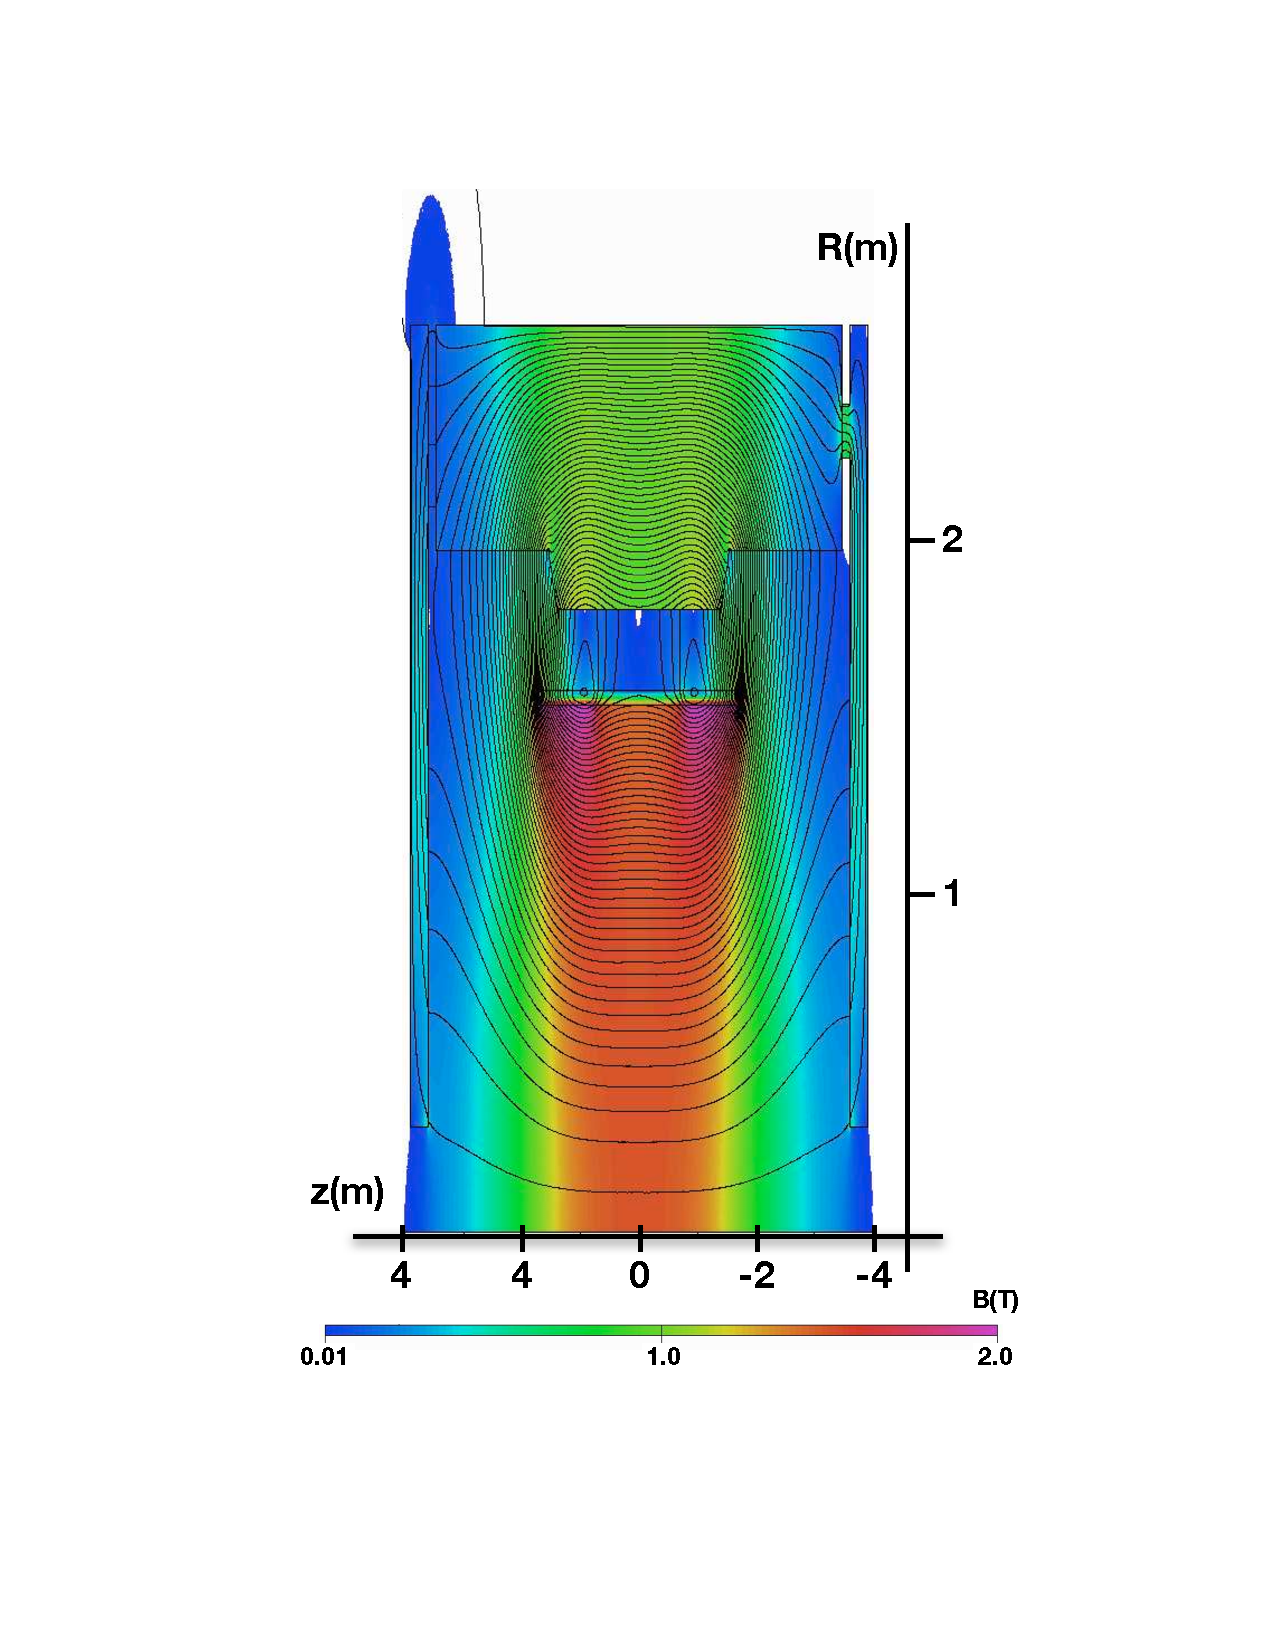
\includegraphics[width=0.5\linewidth,height=0.4\textwidth]{figs/2DSimulation.pdf}
    \caption{2D Opera simulations of the sPHENIX setup}
    \label{Opera2D}
  \end{center}
\end{figure}

These 2D simulations assume a rotational symmetry of the setup and are
a starting point for GEANT4 detector and physics simulations.

As the field depends on the
dimensions and shape of the return yoke, which is not completely symmetric, 
and specifically on the distance of the two
plug-doors with the beam openings, more detailed 3D simulation
are necessary. These can also be used to calculate the forces on the
solenoid. Apart from the mechanical forces due to the
cooldown, the dimensions and shape of the yoke as well as the position
of the coil within the return yoke creates
sizeable forces  on the coil.

\begin{figure}[]
  \begin{center}
    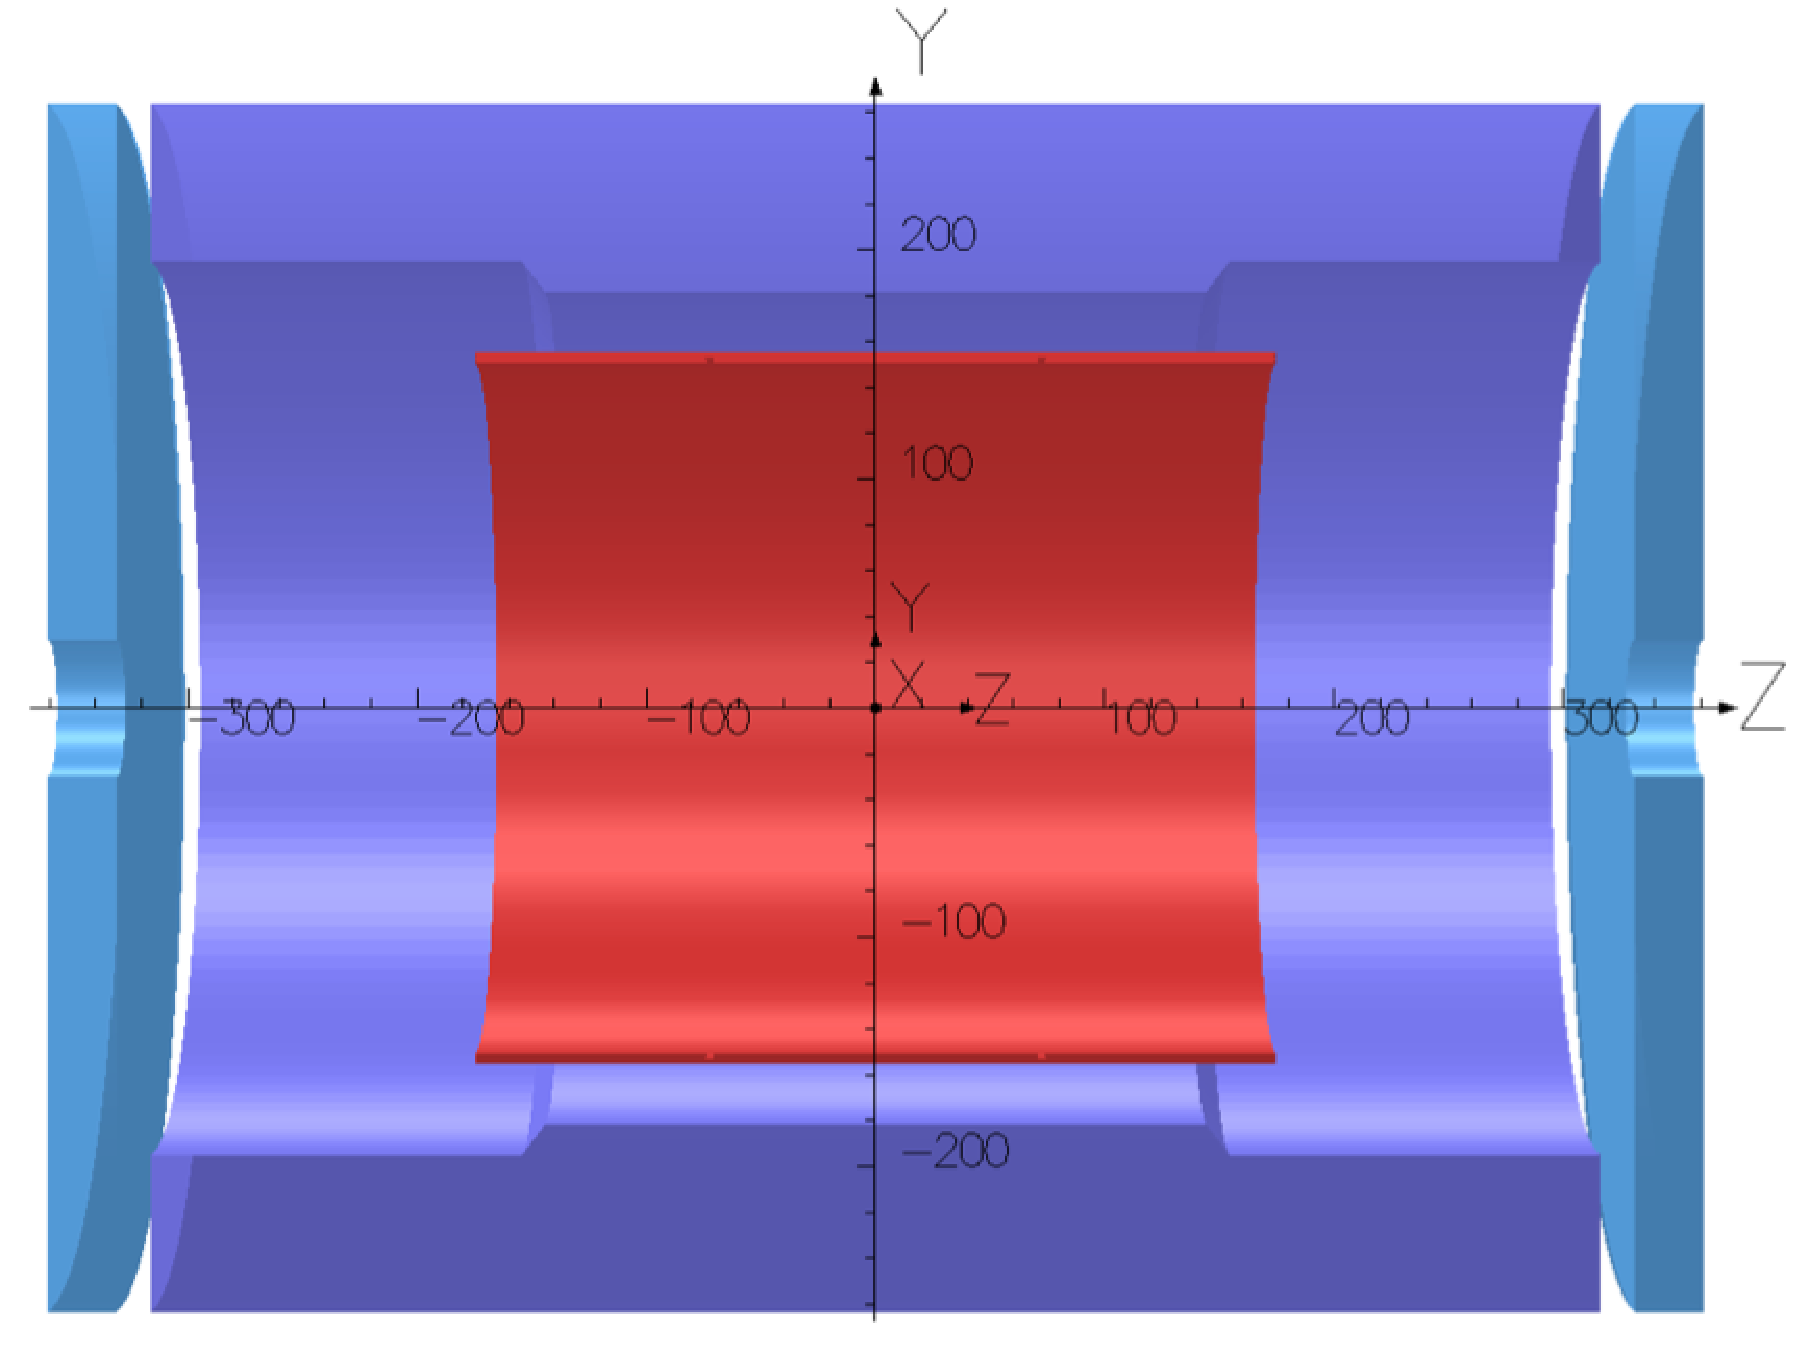
\includegraphics[width=0.5\linewidth, height=0.3\textwidth]{figs/Magnet3DModel.pdf}
    \caption{3D Opera Model}
    \label{Opera2D}
  \end{center}
\end{figure}

The plate struture of the return yoke is a challenging setup for the
finite-element analysis. To simplify the simulations the return yoke
was first replaced by a solid cylinder of magnet steel with the appropriate
density to allow for the scintillator gaps in the real design. 

\begin{figure}[]
  \begin{center}
    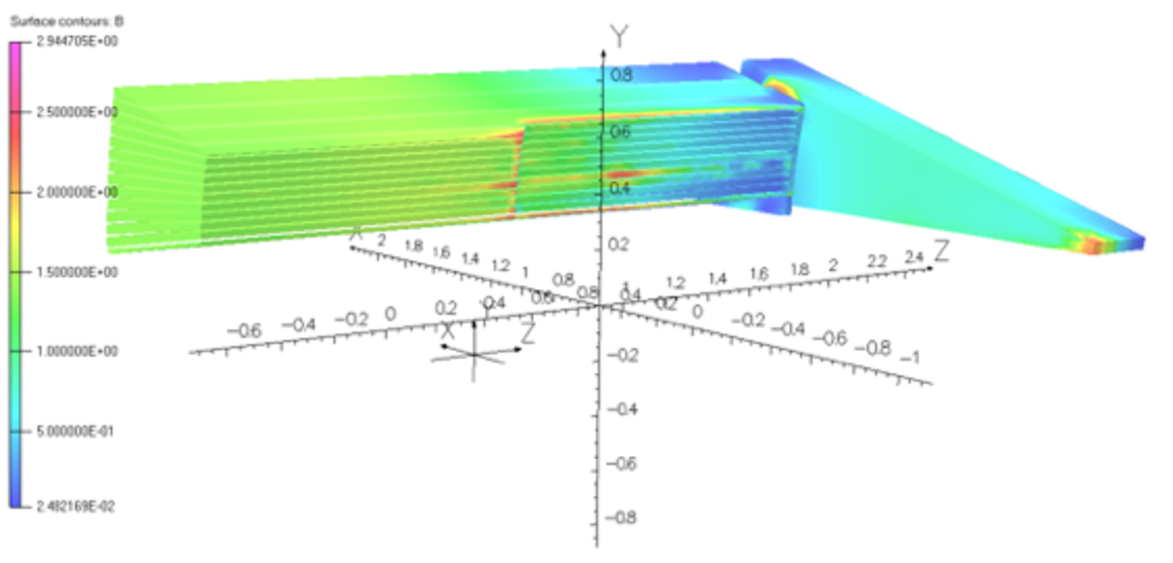
\includegraphics[width=0.5\linewidth, height=0.3\textwidth]{figs/FieldHCalPlateDetail.pdf}
    \caption{Detail of the field in the HCal plates}
    \label{Opera2D}
  \end{center}
\end{figure}



\section{Field Mapping}
\label{Field_Mapping}

To achieve the required momentum resolution the solenoid field has to
be mapped in detail, specially towards the edges of the tracker
acceptance where deviations from the ideal solenoidal field are
expected.

There will be three separate monitoring and mapping tasks. The low and
full field tests scheduled for late 2015 and 2016 will be just a
monitoring task where we plan to use hall probes that had been used
for the PHENIX magnet mapping. For the low field test, with a maximal
current of 100A, a series of probes will be placed inside the solenoid
and read out by a Keithley 7002 Switch System. These monitoring probes
provide a few comparison points to field calcualations.

For the full field test at a current of 4596A, more of the original probes together
with high resolution NMR probes will be installed in the magnet. The
NMR probes will provide a high resolution measurement of the field and
will later be installed as permanent monitoring probes in the final setup.

A detailed field map for track reconstruction has to be measured once
the final return yoke is complete, together with the plug doors. The
shape of the field depends very much on the shape and material of the
yoke. We will employ the CERN magnet mapping group which has years of
experience in field mapping. This group mapped e.g. the STAR magnet
\cite{Bergsma:2002ac} 
and more recent the CMS \cite{Klyukhin:2011df} and ATLAS \cite{Aleksa:2008zza} magnets.

\begin{figure}[]
  \begin{center}
    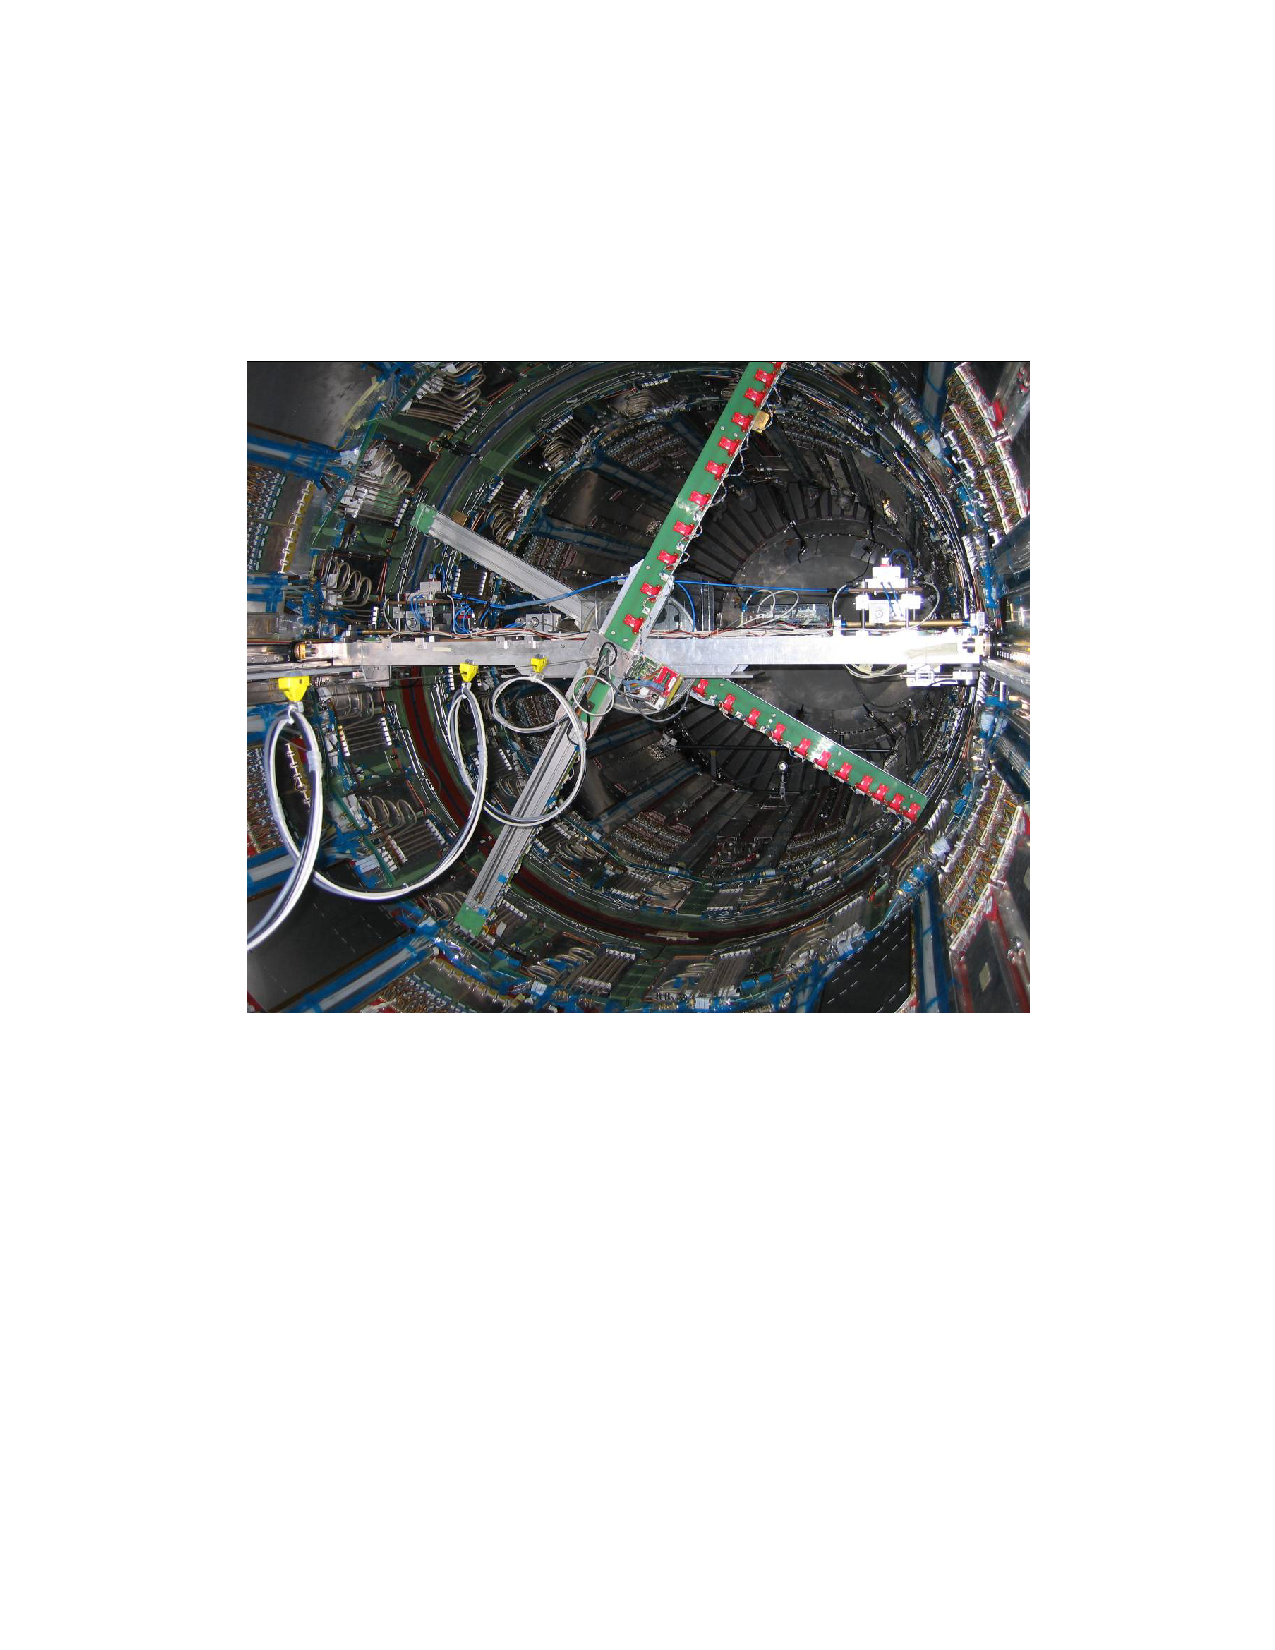
\includegraphics[width=0.5\linewidth, height=0.4\textwidth]{figs/CERNMapper.pdf}
    \caption{The CERN field mapper installed in the ATLAS solenoid}
    \label{CERNMapper}
  \end{center}
\end{figure}

Over the years the hardware has been improved and currently uses
compact hall probes which measure three orthogonal directions.  

\begin{figure}[]
  \begin{center}
    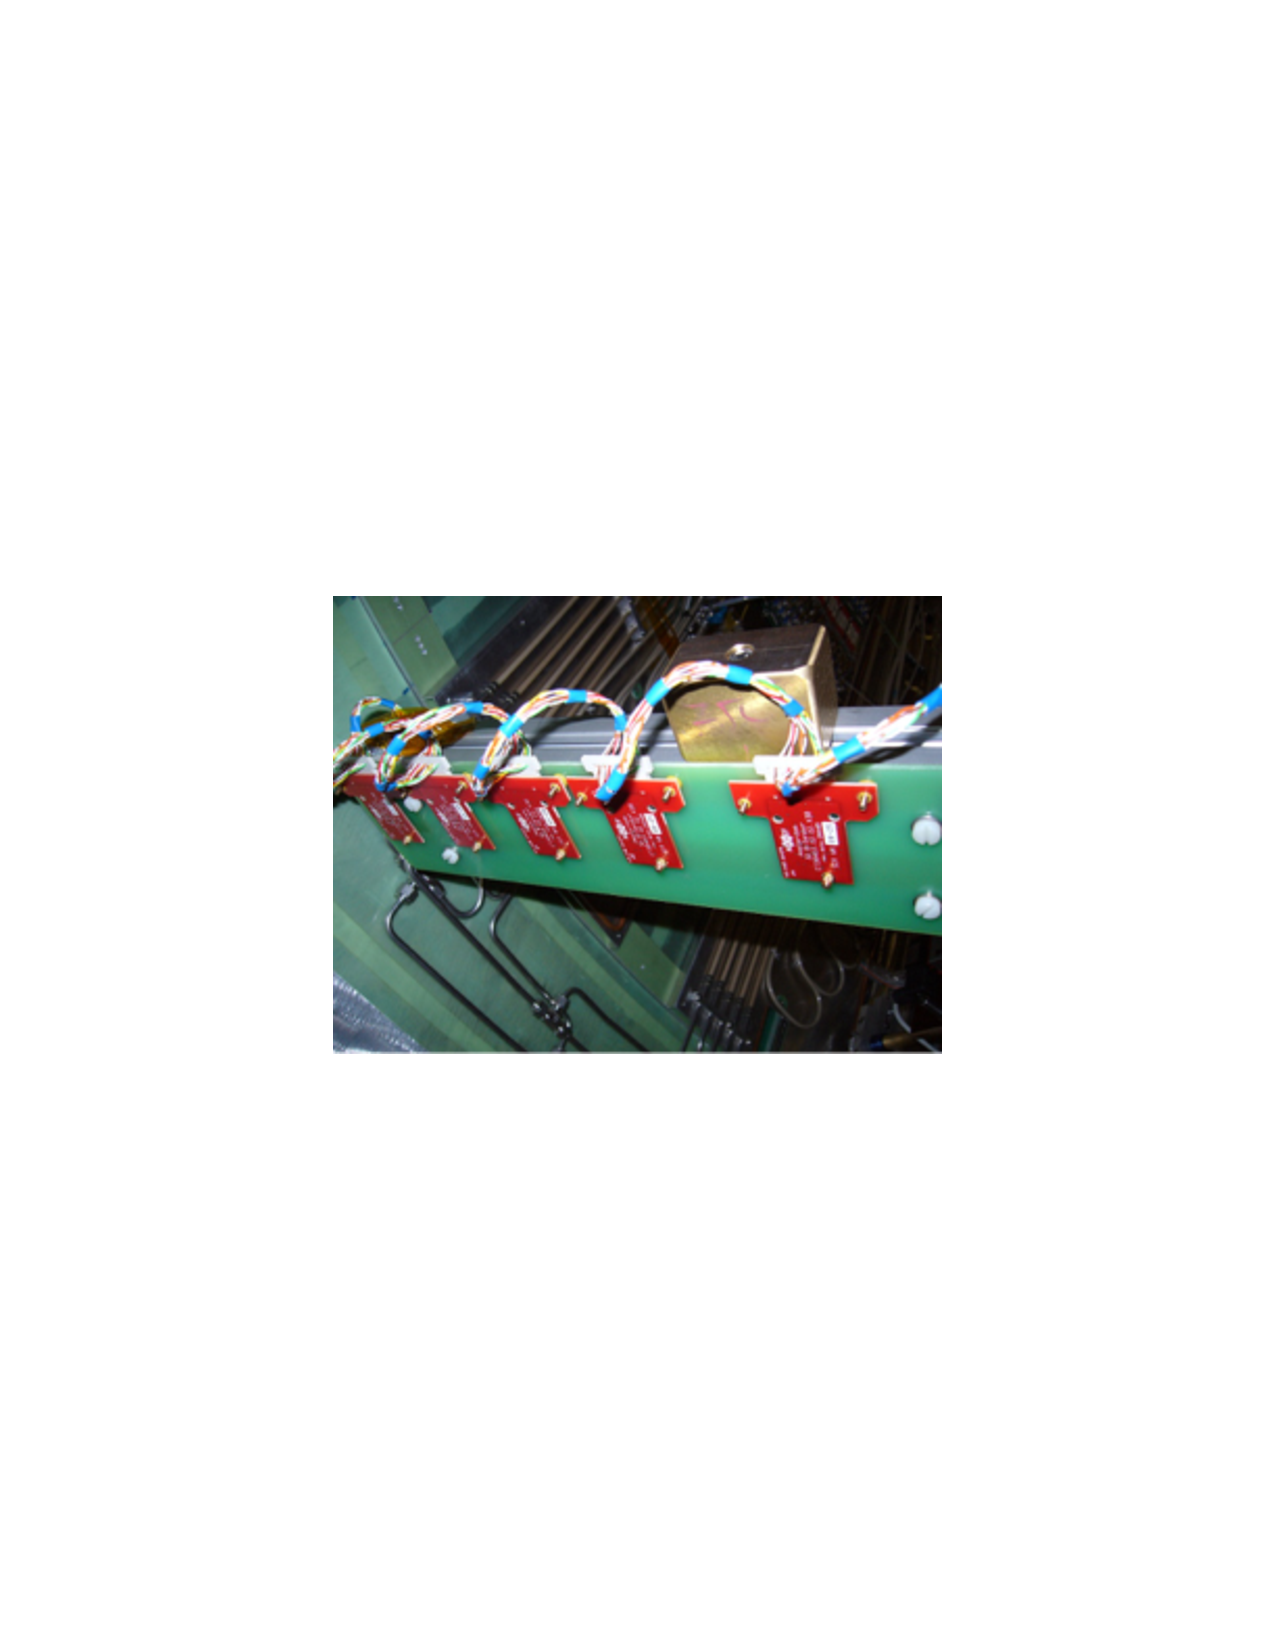
\includegraphics[width=0.5\linewidth, height=0.3\textwidth]{figs/CERNMapperDetail.pdf}
    \caption{Detail of the CERN field mapper, the red tabs are the 3D
    Hall sensors}
    \label{CERNMapperDetail}
  \end{center}
\end{figure}

The CERN group will ship, install and setup the device in the
solenoid, in total the mapping will take about 2 weeks plus analysis
time. This field map will then be compared to 3D OPERA calcuations and
translated into a three dimensional field map that will be used for
tracking and further detector simulations.

Once you cite references, delete this text being used
to avoid a BibTeX error~\cite{Adare:2999ux}.